\documentclass[a4paper,10pt]{article}
\usepackage{indentfirst}
\usepackage[utf8]{inputenc}
\usepackage{fancyhdr}
\usepackage{array,pdflscape}
\usepackage{makecell}
\usepackage{pgfplots}
\pgfplotsset{compat=1.15}


\pagestyle{fancy}
\fancyhf{}
\fancyhead[LE,RO]{Mocanu Viorel Gabriel}
\fancyhead[RE,LO]{Notiuni de teorie pentru clasa a 	\rom{5}-a}
\fancyfoot[CE,CO]{-\thepage-}


\makeatletter
\newcommand*{\rom}[1]{\expandafter\@slowromancap\romannumeral #1@}
\makeatother


\renewcommand{\headrulewidth}{2pt}
\renewcommand{\footrulewidth}{1pt}
\renewcommand{\contentsname}{Cuprins}

\setlength{\parindent}{2em}




\begin{document}
	
	\tableofcontents
	\newpage
	
	\section{Numere naturale}
	\subsection{Scrierea si citirea numerelor naturale}
	
	Cu totii suntem familiari cu numerele naturale, inca de cand suntem la gradinita folosim aceste numere, fara insa a le numi numere naturale. Ele sunt instinctive si le folosim mereu cu gandul de a numerota lucrurile de zi cu zi.
	
	In scrierea unui numar natural, vor aparea cel mult zece simboluri pe care noi le numim \textbf{cifre arabe}. Acestea sunt: 0,1,2,3,4,5,6,7,8,9. Acest mod de scriere a unui numar natural se numeste scriere in \textbf{baza zece}.
	
	\textbf{Un numar natural de doua cifre} se reprezinta prin scrierea $\overline{ab}$, unde a si b desemneaza cifre si a $\neq$ 0. Adica: $\overline{ab}$ = $a\cdot10+b$
	
	Exemple: a) $17 = 1\cdot10+7$  \hspace{2pt} b) $69 = 6\cdot10+9$.
			
	\textbf{Un numar natul de trei cifre} se reprezinta prin scrierea $\overline{abc}$, unde a,b si c desemneaza cifre si $a\neq0$. Adica : $\overline{abc}$ = $a\cdot100+b\cdot10+c$
	
	Exemple: a) $148=1\cdot100+4\cdot10+8$ \hspace{2pt} b) $903=9\cdot100+0\cdot10+3$
	
	\textbf{Numerele naturale scrise in ordinea: 0,1,2.. formeaza sirul numerelor naturale.}
	
	Daca n este un numar natural oarecare, atunci $n-1$ este predecesorul sau, $n+1$ este succesorul sau, iar numerele $n-1$ si n, respectiv n si $n+1$ se numesc numere consecutive.

	Pentru a citi un numar natural, scris in baza 10, se grupeaza cifrele cate trei, de la dreapta la stanga. Aceste grupe sunt numite clase. Fiecare clasa se compune din: unitati, zeci si sute.
			 
	\begin{table}[htb]
		\centering
		\begin{tabular}{|p{0.5cm}|p{0.5cm}|p{0.8cm}|p{0.5cm}|p{0.5cm}|p{0.8cm}|p{0.5cm}|p{0.5cm}|p{0.8cm}|p{0.5cm}|p{0.5cm}|p{0.8cm}|}
			\hline
			sute       & zeci       & unitati       & sute       & zeci       & unitati      & sute     & zeci     & unitati     & sute       & zeci      & unitati      \\ \hline
			\multicolumn{3}{|c|}{Clasa miliardelor} & \multicolumn{3}{c|}{Clasa milioanelor} & \multicolumn{3}{c|}{Clasa miilor} & \multicolumn{3}{c|}{Clasa unitatilor} \\ \hline
		\end{tabular}
	\end{table}
	
	
	Exemple: 
	
	a) 2 843 103 - doua milioane opt sute patruzeci si trei de mii o suta trei
	
	b) 675 021 432 000 - sase sute saptezeci si cinci de miliarde doua zeci si unu de milioane patru sute treizeci si doua de mii\\
	
	
	\textbf{\underline{Cifre romane}}
	
	In Europa cifrele arabe au patruns mai tarziu, erau folosite urmatoarele simboluri: \rom{1}, \rom{5}, \rom{10}, \rom{50}, \rom{100}, \rom{500}, \rom{1000} numite \textbf{cifre romane}.
	Bineinteles ca aceste simboluri au corespondenta cu numerele naturale:
	 
		\rom{1} = 1 
		\rom{5} = 5 
		\rom{10} = 10
		\rom{50} = 50
		\rom{100} = 100
		\rom{500} = 500
		\rom{1000} = 100
	
	\textbf{Reguli de calcul cu cifrele romane}
	
	1. O cifra cu o valore mai mica sau egala scrisa la dreapta uneia cu o valoare mai mare indica o suma.
	
	Exemplu: $\rom{13} = 10 + 1 + 1 + 1 = 13$
	
	2. O cifra cu o valoara mai mica scrisa la stanga uneia cu o valoare mai mare indica o diferenta.
	
	Exemplu: $\rom{90} = 100 - 10 = 90$
	
	3. Cifrele \rom{1}, \rom{10}, \rom{100}, \rom{1000} pot fi scrise consecutiv de cel mult trei ori.
	
	4. Nu se pot repeta consecutiv cifrele V,L,D si nu se pot scadea.
	

	\subsection{Compararea, ordonarea si aproximarea numerelor naturale}
	
	\textbf{Axa numerelor naturale} este o dreapta pe care se fixeaza un punct O, numit \textbf{origine}, un sens si un segment, numit \textbf{unitate de masura}. In acest fel fiecarui numar natural ii corespunde pe axa un punct.\\
	
	\begin{figure}[htb]
	\centering
	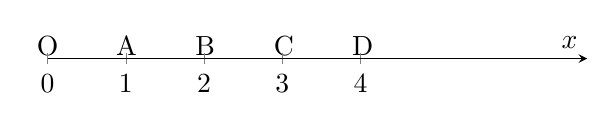
\begin{tikzpicture}
	\node (O) at (0,3){O};
	\node (A) at (1,3){A};
	\node (B) at (2,3){B};
	\node (C) at (3,3){C};
	\node (C) at (4,3){D};
	\label{Fig 1};
	\begin{axis}[
	xlabel={$x$},
	axis x line=center,
	axis y line=none,
	symbolic x coords={0,$1$, $2$, $3$, $4$},
	xmin={[normalized]0},
	xmax={[normalized]6.9},
	xtickmax={[normalized]4},
	xtick distance=1,
	ymin=0,ymax=0% <- added
	]
	\end{axis}
	\end{tikzpicture}
	\end{figure}
	\textbf{\underline{Observatii:}}
	
	\begin{itemize}
		\item Orice nu
		\item
		\item 
	\end{itemize}
	


	

	\section{Operatii cu numere naturale}
	\subsection{Adunarea numerelor naturale}
	\subsection{Scaderea numerelor naturale}
	\subsection{Inmultirea numerelor naturale}
	\subsection{Impartirea numerelor naturale}
	\subsection{Teorema impartirii cu rest}
	\subsection{Ordinea efectuarii operatiilor}
	\subsection{Ridicarea la putere a unui numar natural}
	\subsection{Compararea si ordonarea puterilor}
	\subsection{Operatii cu puteri}
	\section{Divizivilitatea numerelor naturale}
	\subsection{Divizor}
	\subsection{Multiplu}
	\subsection{Divizibilitatea 2,3,5,10}
	\section{Ecuatii si inecuatii}
	\subsection{Media aritmetica}
	\subsection{Ecuatii}
	\subsection{Inecuatii}
	\section{Multimi}
	\subsection{Multime}
	\subsection{Relatii intre multimi}
	\subsection{Multimi finite si multimi infinite}
	\subsection{Operatii cu multimi}
	\section{Fractii ordinare}
	\subsection{Fractie}
	\subsection{Procent}
	\subsection{Fractii echivalente}
	\subsection{Amplificarea si simplificarea fractiilor}
	\subsection{Adunarea si scaderea unor fractii ordinare}
	
	
	
	
\end{document}